%==============================================================================
% Anexos
%==============================================================================

\section{Diagrama de arquitectura del sistema}\label{sec:anexo-diagrama-arquitectura}

El Anexo~A referencia los diagramas de la arquitectura propuesta en notación UML. Los diagramas de despliegue y de secuencia se incluyen como figuras de la \autoref{sec:arquitectura}, de modo que no se reproducen nuevamente aquí; el diagrama de componentes se incluye como Figura~\ref{fig:componentes} de la \autoref{sec:arquitectura}. Los tres artefactos y el cronograma del estudio, que se reproduce aquí, son:

\begin{itemize}
  \item \textbf{Diagrama de despliegue} (Figura~\ref{fig:despliegue}, \autoref{sec:arquitectura}): los cinco componentes principales (N8N, FastAPI, PostgreSQL, Gemini~3.6 Flash, Twilio), el proxy inverso Nginx que, en el diseño, provee terminación TLS~1.2/1.3 en el perímetro del sistema (no incluido en el despliegue publicado), y las relaciones de comunicación entre ellos. Fuente versionada: \texttt{docs/diagrams/despliegue.md}.
  \item \textbf{Diagrama de secuencia} (Figura~\ref{fig:secuencia}, \autoref{sec:arquitectura}): flujo extremo a extremo de un incidente desde su recepción en el canal de correo electrónico hasta la confirmación al usuario, incluyendo las interacciones con el clasificador híbrido y la base de datos. Fuente versionada: \texttt{docs/diagrams/secuencia.md}.
  \item \textbf{Diagrama de componentes} (Figura~\ref{fig:componentes}, \autoref{sec:arquitectura}): organización interna del módulo Python por capas (routes, services, repositories, models, classifiers), con sus dependencias y relaciones. Fuente versionada: \texttt{docs/diagrams/componentes.md}.
  \item \textbf{Cronograma} (Figura~\ref{fig:cronograma}, \autoref{subsec:conexion-scrumban}): construcción, campañas de medición y versión del modelo evaluada, con la procedencia de cada fecha. Fuente versionada: \texttt{docs/diagrams/cronograma.md}.
\end{itemize}

Los diagramas se generan a partir de fuentes Mermaid versionadas en formato \texttt{.md} en el directorio \texttt{docs/diagrams/} del repositorio y se renderizan a imágenes PNG para su inclusión en el documento \parencite{Gomez2026_repositorio}.

\begin{figure}[htbp]
\centering
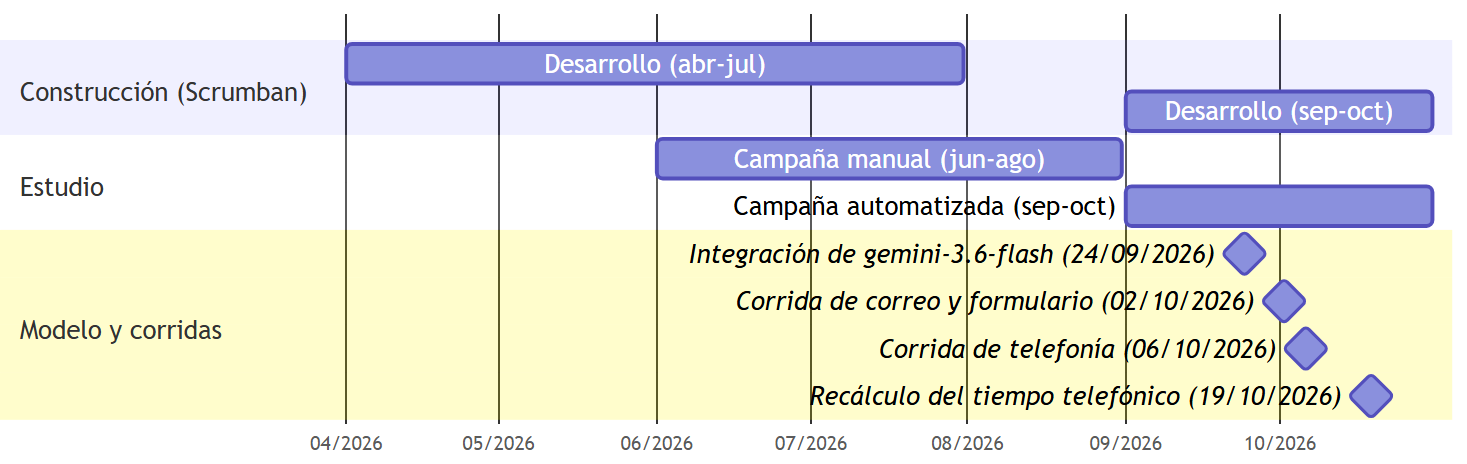
\includegraphics[width=\textwidth,height=0.28\textheight,keepaspectratio]{cronograma}
\caption{Cronograma de la construcción, las campañas y la versión del modelo (barras con precisión de mes; hitos, de día). Fuente: historial del repositorio y confirmación de los autores (9-10-2026).}
\label{fig:cronograma}
\end{figure}

\section{Repositorio de código fuente}\label{sec:anexo-repositorio}

El código fuente del módulo Python, los scripts de migración de la base de datos PostgreSQL gestionados mediante Alembic, los archivos de configuración del despliegue en contenedores Docker y los flujos de integración continua sobre GitHub Actions se encuentran disponibles en el repositorio público del proyecto \parencite{Gomez2026_repositorio}, accesible en \url{https://github.com/lucaGomezB/Automatizacion-de-Mesa-de-Ayuda-N8N}. El commit de referencia para la versión entregada al jurado se identifica con el tag anotado \texttt{v1.2.1}, creado sobre el commit definitivo del repositorio.

El hash completo de ese commit es \texttt{\small 509ffff105c21fed0c07cbf9a46245ba6c53e0e1}, que constituye la referencia verificable de la versión corregida.

La estructura del repositorio separa el módulo de procesamiento (\texttt{App/Backend/}, con la aplicación FastAPI, las migraciones Alembic y las pruebas), la interfaz de usuario (\texttt{App/Frontend/}, React con TypeScript), la definición del flujo de orquestación (\texttt{n8n/workflow.json}), los artefactos de evaluación (\texttt{evaluation/}), el corpus pseudonimizado (\texttt{data/}), los scripts auxiliares (\texttt{scripts/}) y la documentación (\texttt{docs/}), junto con las especificaciones de los changes (\texttt{openspec/}) y los archivos de orquestación local \texttt{docker-compose.yml} y \texttt{Makefile}. El archivo \texttt{README.md} describe esta organización y reúne las instrucciones detalladas para el despliegue local en menos de 15 minutos, por lo que constituye el punto de entrada al código fuente disponible en el repositorio público \parencite{Gomez2026_repositorio}.

\section{Esquema de base de datos}\label{sec:anexo-esquema-bd}

El esquema completo de la base de datos PostgreSQL se documenta mediante scripts SQL versionados que definen las siete entidades descritas en la Tabla~\ref{tab:entidades} de la \autoref{sec:arquitectura}, las restricciones de integridad referencial (claves foráneas con eliminación en cascada condicional), los índices secundarios sobre los atributos de búsqueda frecuente (fecha de creación, sector responsable y estado actual del ticket), y la generación de los identificadores de incidente. Las migraciones incrementales se gestionan mediante Alembic, lo que permite reproducir el estado de la base en cualquier punto histórico del desarrollo y revertir cambios cuando resulte necesario.

La migración inicial incluye la creación de las tablas de catálogo (\texttt{sector}, \texttt{estado}, \texttt{canal\_origen}) con sus valores semilla, garantizando que un despliegue nuevo del sistema comience con los datos de referencia correctos. Las migraciones subsiguientes documentan la evolución del esquema durante las etapas de desarrollo descritas en la \autoref{sec:marco-metodologico}.

El diagrama entidad-relación de las siete entidades se incluye como Figura~\ref{fig:er_modelo_datos} de la \autoref{sec:arquitectura}; su fuente Mermaid versionada reside en \texttt{docs/diagrams/er\_modelo\_datos.md}.

\section{Especificación OpenAPI de la interfaz REST}\label{sec:anexo-openapi}

La especificación completa de la interfaz REST se genera automáticamente mediante FastAPI conforme a la versión~3.1 de la especificación OpenAPI \parencite{Tiangolo2024_fastapi}. El documento resultante describe los puntos de entrada listados en la Tabla~\ref{tab:api} de la \autoref{sec:arquitectura}, los esquemas de los cuerpos de solicitud y respuesta validados mediante Pydantic~v2, los códigos de estado posibles para cada método HTTP, y ejemplos representativos para cada caso de uso.

La interfaz se encuentra disponible adicionalmente en formato interactivo a través del componente Swagger UI integrado en el servidor, accesible bajo la ruta \texttt{/docs} durante la ejecución, y en formato estático como archivo \texttt{openapi.json} en el directorio \texttt{docs/} del repositorio. La sincronización entre el código y la especificación estática se verifica automáticamente en el pipeline de integración continua.

La especificación OpenAPI vigente describe 33 puntos de entrada que exponen 41 métodos HTTP y 44 esquemas de datos, agrupados por recurso: autenticación, catálogos, clasificaciones, incidentes, directorio, estadísticas, telefonía, control de costo y salud.

A título ilustrativo, los 44 esquemas de datos comprenden las estructuras de los catálogos, las entidades de dominio y los objetos de respuesta de cada recurso. El esquema \texttt{IncidenteRead}, por ejemplo, expone el identificador del ticket, la descripción pseudonimizada, la prioridad, el sector y los sectores adicionales, el estado, el canal de origen, el reportante, las marcas temporales de ingreso y persistencia, y los indicadores de latencia end-to-end y de latencia anómala, con sus tipos y campos de solo lectura. El detalle exhaustivo de atributos, tipos y ejemplos reside en \texttt{docs/openapi.json}.

\section{Configuración del flujo N8N}\label{sec:anexo-flujo-n8n}

La exportación del flujo de orquestación en formato JSON incluye la totalidad de los 32 nodos configurados, sus parámetros operativos, las credenciales referenciadas mediante identificadores opacos sin exposición de valores, y los conectores entre nodos. El archivo \texttt{n8n/workflow.json} contiene esta exportación. La importación de este artefacto en una instancia limpia de N8N~2.11.2 reproduce íntegramente el comportamiento operativo del sistema, sujeta únicamente a la provisión de las credenciales correspondientes a los servicios externos integrados (servidor IMAP de correo, cuenta Twilio y clave de API de Gemini) mediante el sistema de credenciales nativo de la plataforma.

La Figura~\ref{fig:anexo_flujo_n8n} presenta una reconstrucción esquemática del flujo, derivada de la exportación JSON y agrupada por etapa funcional. Los 29 nodos operativos (más 3 notas adhesivas, 32 nodos en total) se organizan en siete etapas: entrada (triggers), con la recepción de correo por IMAP y los disparadores de telefonía, formulario web y notificación de clasificación; validación y normalización de la información de entrada, incluida la marca de canal y el sellado de ingreso; envío al backend, con la autenticación del operador y la solicitud POST del incidente; ruteo por canal de origen; revisión humana, con la notificación al operador designado y las respuestas de handoff; respuesta y auditoría del ticket; y aviso post-revisión. La parametrización completa de cada nodo reside en \texttt{n8n/workflow.json}.

\begin{figure}[htbp]
\centering
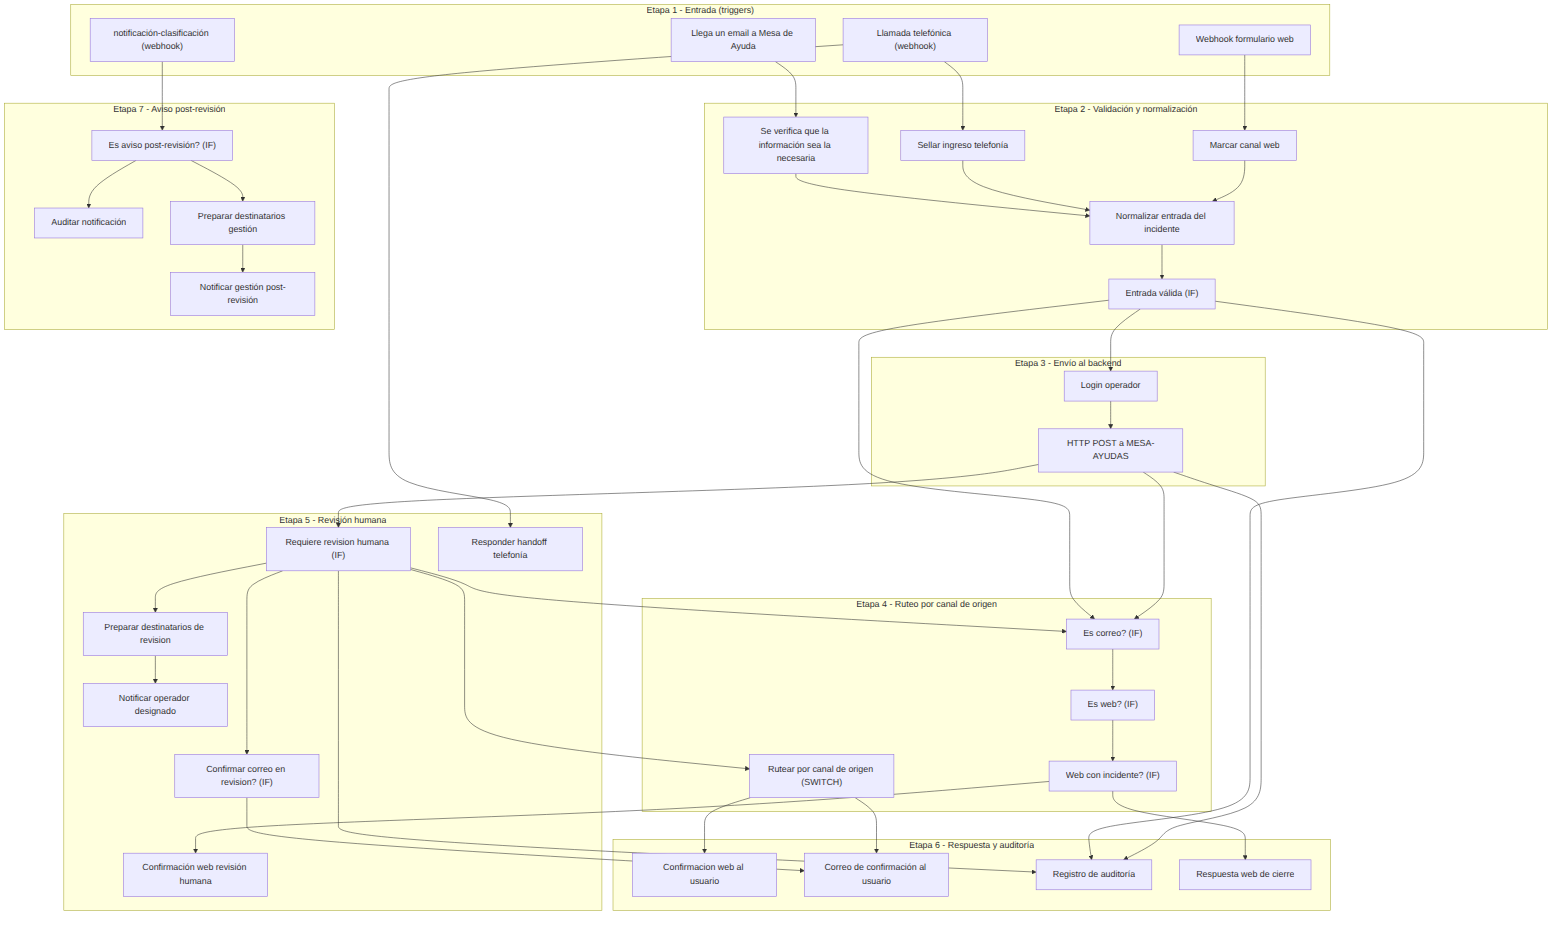
\includegraphics[width=\textwidth]{flujo_n8n}
\caption[Reconstrucción esquemática del flujo de orquestación N8N]{Reconstrucción esquemática del flujo de orquestación N8N: no es una captura de la interfaz; los 29 nodos operativos se agrupan por etapa funcional.}
\label{fig:anexo_flujo_n8n}
\end{figure}

\section{Corpus de validación}\label{sec:anexo-corpus}

El corpus de 200 incidentes utilizado para la validación experimental reside en el repositorio en formato JSON, en su forma pseudonimizada y versionada, bajo la ruta \texttt{data/corpus\_evaluacion\_pseudonimizado.json}. Cada caso incluye el identificador anónimo, la descripción cruda pseudonimizada, el canal de origen, el sector asignado por consenso humano, los sectores adicionales de verdad y el tiempo de registro medido en cada flujo. La categoría predicha por el clasificador y la confianza asociada no forman parte del corpus: se conservan en \texttt{evaluation/predicciones.json}, generado por el framework de evaluación. Se incluyen además las planillas de cronometraje del flujo manual y los registros automáticos generados por el flujo automatizado.

Cada uno de los 200 casos del corpus se compone de siete campos: \texttt{id} (identificador anónimo, por ejemplo \texttt{R001}), \texttt{descripcion} (texto pseudonimizado, con los identificadores personales reemplazados por etiquetas genéricas como \texttt{[EMAIL]}, \texttt{[TELEFONO]}, \texttt{[HOST]} y \texttt{[PERSONA]}), \texttt{canal\_origen} (correo electrónico, formulario web o llamada telefónica), \texttt{sector\_asignado} (sector principal de verdad, exactamente uno de los cinco sectores canónicos), \texttt{sectores\_adicionales} (sectores de verdad complementarios, sin repetir el asignado), \texttt{tiempo\_manual\_s} (tiempo de clasificación manual, en segundos) y \texttt{tiempo\_automatizado\_s} (tiempo del sistema automatizado, en segundos). El corpus completo reside en \texttt{data/corpus\_evaluacion\_pseudonimizado.json} y las predicciones del clasificador en \texttt{evaluation/predicciones.json}.

Por razones de privacidad y en cumplimiento de la Ley~25.326 \parencite{Ley25326_2000}, las descripciones textuales han sido pseudonimizadas previamente a su inclusión en el repositorio público, reemplazando nombres propios, direcciones de correo y otros identificadores personales por etiquetas genéricas.

\section{Documentación operativa}\label{sec:anexo-documentacion-operativa}

La documentación operativa del sistema, que reúne los procedimientos de despliegue, configuración, respaldo y restauración, monitoreo y respuesta ante incidentes operativos, se versiona en el repositorio junto con el código fuente; el runbook operativo reside en \texttt{docs/operational-guide.md}.

\section{Especificación del prompt de Gemini 3.6 Flash}
\label{anexo:H}

Este anexo documenta la especificación del prompt enviado al modelo \texttt{gemini-3.6-flash} (Gemini~3.6 Flash en el texto) y los parámetros de configuración de la inferencia. El prompt se mantiene en el repositorio bajo \texttt{docs/prompt\_gemini.txt} y es único para los tres canales de entrada.

\subsection{Estructura y contenido del prompt}\label{subsec:anexo-estructura-prompt}

El prompt sigue una estructura fija en español organizada en cinco componentes funcionales y un conjunto de reglas de desambiguación:

\begin{enumerate}
  \item \textbf{Instrucción de rol}: define que el modelo actúa como agente especializado en clasificación de incidentes técnicos en español rioplatense, lo que ancla el comportamiento en el dominio y el dialecto del estudio.
  \item \textbf{Definición de categorías}: presenta los cinco sectores canónicos con sus \emph{strings} exactos (sensibles a mayúsculas y sin tildes), un ámbito descriptivo por sector y un ejemplo representativo extraído del dominio real por cada uno.
  \item \textbf{Formato de respuesta}: solicita un JSON válido con exactamente dos campos, \texttt{categoría} (uno de los cinco valores canónicos) y \texttt{confianza} (número entre 0,0 y 1,0), sin texto adicional, comentarios ni explicaciones.
  \item \textbf{Lógica de decisión}: indica analizar la descripción y asignar una categoría única entre las cinco opciones; ante elementos de múltiples categorías, elegir la dominante.
  \item \textbf{Validación sintáctica}: exige validar la corrección sintáctica del JSON antes de devolverlo y reducir la confianza cuando no sea posible clasificar con seguridad.
  \item \textbf{Reglas de desambiguación de frontera}: las acciones sobre aplicaciones o sistemas operativos (acceder, iniciar sesión, abrir una aplicación) se orientan a \texttt{Soporte Tecnico Software}; los dispositivos físicos y su digitalización (escáner, impresora, periférico, error de digitalización) a \texttt{Soporte Tecnico Hardware}; y la infraestructura y los servicios de plataforma (servidor, red, SMTP, VM) a \texttt{Sistemas}. Estas reglas corrigen casos de frontera medidos sobre el corpus.
\end{enumerate}

\subsection{Parámetros de configuración}\label{subsec:anexo-parametros-config}

La invocación del modelo se realiza mediante el SDK \texttt{google-genai} (\texttt{>=2.20.0}), con los hiperparámetros que resume la Tabla~\ref{tab:anexo_gemini_params}, que corresponden a la configuración adoptada para el despliegue y no al resultado de una calibración documentada frente a valores alternativos (\autoref{subsec:capa-procesamiento}).

\begin{table}[htbp]
\small
\centering
\caption{Parámetros de configuración de la inferencia con \texttt{gemini-3.6-flash}.}
\label{tab:anexo_gemini_params}
\begin{tabular}{@{}>{\raggedright\arraybackslash}p{3.0cm} >{\raggedright\arraybackslash}p{2.6cm} >{\raggedright\arraybackslash}p{8.4cm}@{}}
\toprule
Parámetro & Valor & Justificación \\
\midrule
\texttt{temperature} & 0,3 & Valor bajo que reduce la variabilidad de la generación y mejora la consistencia en tareas de clasificación determinística. \\
\texttt{top\_p} & 0,9 & \emph{Nucleus sampling} que admite variantes léxicas válidas en español rioplatense sin sacrificar coherencia. \\
\texttt{max\_tokens} & 100 & Límite suficiente para la respuesta JSON, con margen ante variaciones y sin truncamiento. \\
\texttt{candidate\_count} & 1 & Respuesta única sin remuestreo, que acota la latencia del procesamiento en tiempo real. \\
\texttt{safety\_settings} & Parcialmente desactivados & Desactiva filtros que podrían rechazar descripciones legítimas de incidentes, manteniendo los filtros contra contenido verdaderamente tóxico. \\
\texttt{timeout} & 30 segundos por intento; 60 segundos en total & Límite de latencia por intento del backend al modelo (hasta dos reintentos ante fallas transitorias, dentro de un presupuesto total de 60 segundos por clasificación; no son reintentos de N8N al backend); al agotarse, el clasificador devuelve confianza 0,0 y marca el caso para revisión humana. \\
Umbral de revisión humana & 0,70 & Confianza mínima de una respuesta del modelo para no marcarla para revisión; no se aplica a la etapa determinística (\autoref{subsec:subsistema-clasificacion}). \\
SDK & \texttt{google-genai} \texttt{>=2.20.0} & Versión vigente al momento del estudio, documentada para reproducibilidad. \\
\bottomrule
\end{tabular}
{\footnotesize\textit{Fuente:} elaboración propia a partir de la documentación del SDK \texttt{google-genai}.\par}
\end{table}

\subsection{Validación de la respuesta}\label{subsec:anexo-validacion-respuesta}

Antes de aceptar la respuesta del modelo, el módulo de clasificación valida que el texto sea JSON parseable, que contenga exactamente las claves \texttt{categoría} y \texttt{confianza}, que la categoría sea uno de los cinco valores canónicos y que la confianza sea un número en el intervalo \([0{,}0, 1{,}0]\). Si cualquiera de estas condiciones falla, se registra la excepción, se asigna confianza 0,0, se marca el incidente para revisión humana y no se propagan estados inconsistentes a la base de datos. Este procedimiento garantiza la confiabilidad operativa frente a errores de formato o alucinaciones del modelo. El Listado~\ref{lst:validar-gemini} resume la rutina de validación.

\begin{lstlisting}[caption={Validación de la respuesta de Gemini (resumen).},label={lst:validar-gemini}]
def validar_respuesta_gemini(response_text: str) -> tuple[bool, dict]:
    try:
        data = json.loads(response_text)
    except json.JSONDecodeError as e:
        return False, {"error": f"JSON invalido: {e}"}
    if "categoria" not in data:
        return False, {"error": "Falta campo 'categoria'"}
    if data["categoria"] not in SECTORES_CANONICOS:
        return False, {"error": f"Categoria invalida: {data['categoria']}"}
    if "confianza" not in data:
        return False, {"error": "Falta campo 'confianza'"}
    if not isinstance(data["confianza"], (int, float)) \
            or not (0.0 <= data["confianza"] <= 1.0):
        return False, {"error": f"Confianza invalida: {data['confianza']}"}
    return True, data
\end{lstlisting}

\subsection{Iteración y mejora del prompt}\label{subsec:anexo-iteracion-prompt}

El prompt de la versión evaluada se ajustó de forma iterativa a partir de errores observados en el corpus de validación; no se dispuso de un corpus independiente de preproducción. Las versiones históricas del prompt se conservan en el historial de versiones del repositorio (archivo \texttt{docs/prompt\_gemini.txt}) para auditoría y eventual reversión.

\subsection{Recomendaciones para futuras iteraciones}\label{subsec:anexo-recomendaciones-prompt}

Ante una degradación de las métricas por cambios en el modelo, se recomienda profundizar los ejemplos por clase (de dos a cuatro o cinco), agregar contraejemplos de incidentes limítrofes, especificar umbrales de confianza explícitos, incluir un diccionario de términos clave por categoría y, una vez acumulado un corpus del orden de 5.000 casos etiquetados (referencia indicativa de orden de magnitud, no derivada del corpus actual ni de un cálculo de potencia estadística), migrar a un modelo ajustado específicamente al dominio.

\section{Trazabilidad de las correcciones del dictamen}\label{sec:anexo-trazabilidad}

El registro de correcciones derivado del dictamen evaluador se conserva como artefacto versionado en el repositorio, bajo la ruta \texttt{docs/Tesis/Correcciones/dictamen-correcciones.md}. El documento compila, de forma acumulativa, cada corrección aplicada al manuscrito y las decisiones adoptadas sobre las observaciones que no admitían una resolución inmediata (por ejemplo, la convención estadística del estadístico \emph{W}, la reformulación de la hipótesis principal y el tratamiento de los reintentos como limitación conocida). Se incluye aquí como ejemplo de trazabilidad: cada entrada del registro vincula una observación del dictamen con el archivo y la línea corregidos, de modo que la correspondencia entre la revisión solicitada y la revisión efectuada resulte auditable de extremo a extremo.

El dictamen que motiva las correcciones vigentes es el emitido el 22 de octubre de 2026 sobre la versión de trabajo v10, publicada como \texttt{v1.1.0} y aplicable por igual a \texttt{v1.1.1}. Sus cinco observaciones de fondo (A1 a A5) y sus correcciones de consistencia (B4 a B16) se atendieron mediante changes del repositorio; la \autoref{tab:anexo-trazabilidad} indica, para cada una, el change responsable y las secciones de la tesis donde se la atendió. Cuando una recomendación se dividió en partes, figuran los changes que las atendieron.

\begin{table}[htbp]
\small
\centering
\caption{Recomendaciones del dictamen del 22 de octubre de 2026, change responsable y secciones donde se atendieron.}
\label{tab:anexo-trazabilidad}
\setlength{\tabcolsep}{4pt}
\begin{tabular}{@{}>{\raggedright\arraybackslash}p{1.0cm} >{\raggedright\arraybackslash}p{3.3cm} >{\raggedright\arraybackslash}p{10.6cm}@{}}
\toprule
Rec. & Change & Secciones de la tesis \\
\midrule
A1 & \texttt{c-130} & \autoref{subsec:human-in-the-loop}, \autoref{subsec:subsistema-clasificacion}, \autoref{subsec:construccion-flujo-n8n}, \autoref{subsec:reduccion-intervencion} \\
A2 & \texttt{c-131} & \autoref{subsec:calibracion}, \autoref{tab:bandas}, \autoref{tab:exactitud-etapa-canal}, \autoref{subsec:interpretacion-resultados} \\
A3 & \texttt{c-132} & \autoref{subsec:balance-neto}, \autoref{subsec:implicancias-practicas} \\
A4 & \texttt{c-139}, \texttt{c-138} & \autoref{subsec:nlp-llm}, \autoref{subsec:trabajos-academicos}, \autoref{subsec:calibracion-cascadas}, \autoref{subsec:clasificador-supervisado} \\
A5 & \texttt{c-130}, \texttt{c-144}, \texttt{c-142} & \autoref{subsec:subsistema-clasificacion}, \autoref{subsec:conexion-scrumban}, \autoref{subsec:interpretacion-resultados}, \autoref{subsec:anexo-iteracion-prompt}; \autoref{subsec:sensibilidad-ajustes}, \autoref{subsec:limitaciones-estudio} \\
B4 & \texttt{c-133} & \autoref{tab:cumplimiento-objetivos}, \autoref{subsec:cumplimiento-objetivos} \\
B5 & \texttt{c-133} & \autoref{subsec:hipotesis-trabajo} \\
B6 & \texttt{c-133} & \autoref{subsec:metricas-instrumentos}, \autoref{tab:metricas} \\
B7 & \texttt{c-134}, \texttt{c-131} & \autoref{tab:tiempos-canal}; \autoref{tab:exactitud-etapa-canal} \\
B8 & \texttt{c-131} & \autoref{subsec:metricas-instrumentos}, \autoref{tab:exactitud-etapa-canal} \\
B9 & \texttt{c-135} & \autoref{subsec:gestion-scrumban}, \autoref{subsec:conexion-scrumban}, \autoref{fig:cronograma}, \autoref{subsec:limitaciones-estudio} \\
B10 & \texttt{c-135} & \autoref{sec:resultados}, \autoref{tab:comparativa}, \autoref{tab:trabajos-academicos} \\
B11 & \texttt{c-136} & \autoref{sec:recomendaciones}, \autoref{subsec:calibracion-gate}, \autoref{subsec:medicion-intervencion}, \autoref{subsec:aprendizaje-activo} \\
B12 & \texttt{c-134} & \autoref{subsec:analisis-estadistico}, \autoref{subsec:poblacion-muestra-corpus} \\
B13 & \texttt{c-135}, \texttt{c-134} & \autoref{subsec:cumplimiento-objetivos}; \autoref{subsec:diseno-experimental}, \autoref{subsec:consentimiento-derechos} \\
B14 & \texttt{c-137} & Todo el documento (revisión ortotipográfica) \\
B15 & \texttt{c-139} & \autoref{subsec:cumplimiento}, \autoref{subsec:analisis-estadistico} \\
B16 & \texttt{c-139}, \texttt{c-141} & \autoref{sec:anexo-repositorio} y Referencias bibliográficas \\
\bottomrule
\end{tabular}
\par\smallskip
{\footnotesize\textit{Fuente:} elaboración propia a partir de \texttt{docs/Tesis/Correcciones/dictamen-correcciones.md}.\par}
\end{table}

La trazabilidad interna de dos decisiones que el cuerpo del Capítulo~6 presenta en lenguaje llano se conserva aquí: el retiro de la rama de clasificación telefónica por agente LLM basada en LangChain y el traslado de la superficie de costo al backend corresponden al change \texttt{c-72}. El detalle de ambas decisiones figura en \texttt{docs/Tesis/Correcciones/dictamen-correcciones.md}.

\newpage
